% Created 2022-09-05 Mon 17:33
% Intended LaTeX compiler: pdflatex
\documentclass[smaller]{beamer}\usepackage{listings}
\usepackage{color}
\usepackage{amsmath}
\usepackage{array}
\usepackage[T1]{fontenc}
\usepackage{natbib}
\lstset{
keywordstyle=\color{blue},
commentstyle=\color{red},stringstyle=\color[rgb]{0,.5,0},
literate={~}{$\sim$}{1},
basicstyle=\ttfamily\small,
columns=fullflexible,
breaklines=true,
breakatwhitespace=false,
numbers=left,
numberstyle=\ttfamily\tiny\color{gray},
stepnumber=1,
numbersep=10pt,
backgroundcolor=\color{white},
tabsize=4,
keepspaces=true,
showspaces=false,
showstringspaces=false,
xleftmargin=.23in,
frame=single,
basewidth={0.5em,0.4em},
}
\institute{PhD Student, Section of Biostatistics \\ University of Copenhagen}
\usepackage{natbib, dsfont, pgfpages, tikz,amssymb, amsmath,xcolor}
\bibliographystyle{abbrvnat}
% New operators and commands
\newcommand{\Z}{\mathbb{Z}}
\newcommand{\Q}{\mathbb{Q}}
\newcommand{\R}{\mathbb{R}}
\newcommand{\N}{\mathbb{N}}
\newcommand{\C}{\mathbb{C}}
\renewcommand{\S}{\mathbb{S}}
\newcommand{\blank}{\makebox[1ex]{\textbf{$\cdot$}}}
\newcommand\independent{\protect\mathpalette{\protect\independenT}{\perp}}
\def\independenT#1#2{\mathrel{\rlap{$#1#2$}\mkern2mu{#1#2}}}
\renewcommand{\phi}{\varphi}
\renewcommand{\epsilon}{\varepsilon}
\newcommand*\diff{\mathop{}\!\mathrm{d}}
\newcommand{\weakly}{\rightsquigarrow}
\newcommand\smallO{
  \mathchoice
    {{\scriptstyle\mathcal{O}}}% \displaystyle
    {{\scriptstyle\mathcal{O}}}% \textstyle
    {{\scriptscriptstyle\mathcal{O}}}% \scriptstyle
    {\scalebox{.6}{$\scriptscriptstyle\mathcal{O}$}}%\scriptscriptstyle
}
\newcommand{\midd}{\; \middle|\;}
\newcommand{\1}{\mathds{1}}
\usepackage{ifthen} %% Empirical process with default argument
% \newcommand{\G}[1][]{%
%    \ifthenelse{ \equal{#1}{} }
%       {\ensuremath{\mathbb{G}_n}}
%       {\ensuremath{\mathbb{G}_{#1}}}
% }
% New version:
\newcommand{\G}[2][n]{
{\ensuremath{\mathbb{G}_{#1}}{\left[#2\right]}}
}
\DeclareMathOperator*{\argmin}{\arg\!\min}

% New operators for consistent notation
\newcommand{\V}{\mathrm{Var}} % variance
\newcommand{\measure}[1]{\mathrm{{#1}}} % measure
% \newcommand{\measure}[1]{\textnormal{\textbf{{#1}}}} % measure
\newcommand{\m}[1]{\measure{#1}} % measure shortcut
\newcommand{\eqd}{\stackrel{d}{=}} % equality in distribution
\newcommand{\arrow}[1]{\xrightarrow{\; {#1} \;}}
\newcommand{\arrowP}{\xrightarrow{\; \m{P} \;}} % convergence in probability
\newcommand{\leb}{\lambda} % the Lebesgue measure
\newcommand{\T}{\top} % transpose
\newcommand{\KL}{\ensuremath{D_{\mathrm{KL}}}}

\usepackage{xargs}
% Make it easy to change counterfactual notation:
\newcommandx{\cf}[4][3={}, 4={}]{
  % \ifthenelse{ \equal{#4}{} }
  % {{#1^{#2}}(#3)}
  {\ifthenelse{ \equal{#3}{} }
    {{#1^{#2}}_{#4}}
    {{#1^{#2}}_{#4}(#3)}}
}

% Easily change notation:
\DeclareMathOperator{\TT}{\Psi} % target parameter
\newcommand{\lp}{\mathcal{L}_{\P}^2} % shortcut for lp2 space
\newcommand{\empmeas}{\hat{\mathbb{P}}_n} % empirical measure
\DeclareMathOperator{\E}{\mathbb{E}} % expectation
\renewcommand{\P}{\m{P}} % probability
\newcommand{\ic}{\mathrm{IF}} % influence curve
\newcommand{\est}{\ensuremath{\nu}}
\setbeamertemplate{footline}[frame number]
\beamertemplatenavigationsymbolsempty
\usepackage{appendixnumberbeamer}
\setbeamercolor{gray}{bg=white!90!black}
\setbeamertemplate{itemize items}{$\circ$}
\lstset{basicstyle=\footnotesize\selectfont\ttfamily,keywordstyle=\color{black}}

\renewcommand*\familydefault{\sfdefault}
\itemsep2pt
\usepackage[utf8]{inputenc}
\usepackage[T1]{fontenc}
\usepackage{graphicx}
\usepackage{longtable}
\usepackage{wrapfig}
\usepackage{rotating}
\usepackage[normalem]{ulem}
\usepackage{amsmath}
\usepackage{amssymb}
\usepackage{capt-of}
\usepackage{hyperref}
\usetheme{default}
\author{Anders Munch \newline \small joint work with Thomas Gerds}
\date{September 7, 2022 -- JICI}
\title{Loss functions and cross-validation with censored survival data}
\begin{document}

\maketitle
\begin{frame}{Outline}
\tableofcontents
\end{frame}

\section{Setting and data structure}
\label{sec:org2f6c6ea}
\begin{frame}[label={sec:orgeb4e8b4}]{Data structure and target of inference}
\small
\begin{block}{Survival setting}
\begin{description}
\item[{\(O = (\tilde T, \Delta, X) \sim P \in \mathcal{P}\)}] Oberved data with \(\mathcal{O} = \R_+
  \times \{0,1\} \times \R^p\).
\item[{\(Z = (T, X) \sim Q \in \mathcal{Q}\)}] The distribution \(Q\) (or a feature of it) is of interest.
\end{description}

\hfill
\end{block}

\begin{block}{Parameters of interest}
Low-dimensional feature of \(Q\), e.g., the marginal survival probability \(Q(T > t)\) for a fixed
time horizon \(t \in \R_+\).

\hfill
\end{block}


\begin{block}{Nuisance parameter}
The distribution \(Q\) is identifiable from the observed data distribution \(P\) under coarsening at
random. Without further assumptions we would typically need to estimate the conditional survival
function \(S(t \mid x) = Q(T > t \mid X=x)\) (and/or the conditional censoring distribution).
\end{block}
\end{frame}

\begin{frame}[label={sec:org75ad0a2}]{Cross-validation and super learning for \(S\)}
\pause Most machine learning methods depend on one or more hyperparameters which are typically
chosen using \textbf{cross-validation}.

\vfill

More generally, to build robust estimators we can use \textbf{stacked regression} /
\textbf{super~learning} \citep{breiman1996stacked,van2007super} to select from or combine a
collection candidate estimators/algorithms.

\vfill

A central component for both cross-validation and super learning is the partitioning of data into
training and test folds. A suitable loss function is then used to evaluate the performance of an
estimator in hold-out samples.
\end{frame}

\begin{frame}[label={sec:orgc69e91e}]{Evaluate performance in hold-out samples}
\small

\begin{description}
\item[{\(D\)}] data set \((O_1, \dots, O_n)\)
\item[{\(\mathcal{A}\)}] collection of algorithms for estimating \(S \in \mathcal{S}\)
\item[{\(\nu \in \mathcal{A}\)}] mapping \(D \longmapsto \est(D) = \hat S \in
  \mathcal{S}\)
\item[{\(L\)}] loss function, \(L \colon \mathcal{S} \times \mathcal{O} \rightarrow \R_+\)
\end{description}

\vfill
To evaluate the performance of \(\est \in \mathcal{A}\) let
\begin{description}
\item[{\(D_1, \dots, D_K\)}] partition of the data set \(D\)
\item[{\(D_{-k}\)}] the \(k\)'th training sample, \(D_{-k} = D \setminus
  D_{k}\), \(k=1, \dots, K\)
\end{description}

and evaluate for all \(i = 1, \dots, n\),
\begin{equation*}
L(\est(D_{-k}), O_i),
\quad \text{for all} \quad O_i \in D_k.
\end{equation*}
Averaging these values gives us an estimate of the expected loss of the algorithm \(\nu \in
\mathcal{A}\), and we can then pick the one with lowest expected loss. Alternatively, we can use
these value to combine all algorithms into a super learner.
\end{frame}


\section{Loss functions and hold-out samples for survival data}
\label{sec:org88e0534}

\begin{frame}[label={sec:orga8896fd}]{The partial likelihood and hold-out samples}
\small A popular choice for training survival models is the negative partial log-likelihood loss.
Assuming conditional independence between the outcome and the censoring given the covariates, the
observed data factorizes as
\begin{equation*}
  \ell(P, O) = \ell_t(S, O) \cdot \ell_c(G, O) \cdot \ell_0(h, O),
\end{equation*}
where \(G \in \mathcal{G} \) denotes the censoring mechanism and $h$ the marginal distribution of
the baseline covariates. The negative partial log-likelihood for the component \(S\) is
\begin{equation*}
  - \log \ell_t(S, O)
  = -
  \left\{
    (1-\Delta) \log S(\tilde T \mid X)
    + \Delta \log f_S(\tilde T \mid X)
  \right\},
\end{equation*}
where \(f_S\) is the conditional density corresponding to \(S\). \vfill

However, in continuous time this loss function is unsuitable for evaluating performance of most
common survival estimators in hold-out samples, because (a.s.)
\begin{equation*}
  f_{\hat S}(\tilde T_i \mid X_i) = 0
  \quad \text{when} \quad
  \hat S =\est(D_{-k})
  \quad \text{and} \quad
  (\tilde T_i, \Delta_i, X_i) \in D_k.
\end{equation*}
\end{frame}

\begin{frame}[label={sec:org90cecce}]{Illustration}
\begin{onlyenv}<1>
\begin{center}
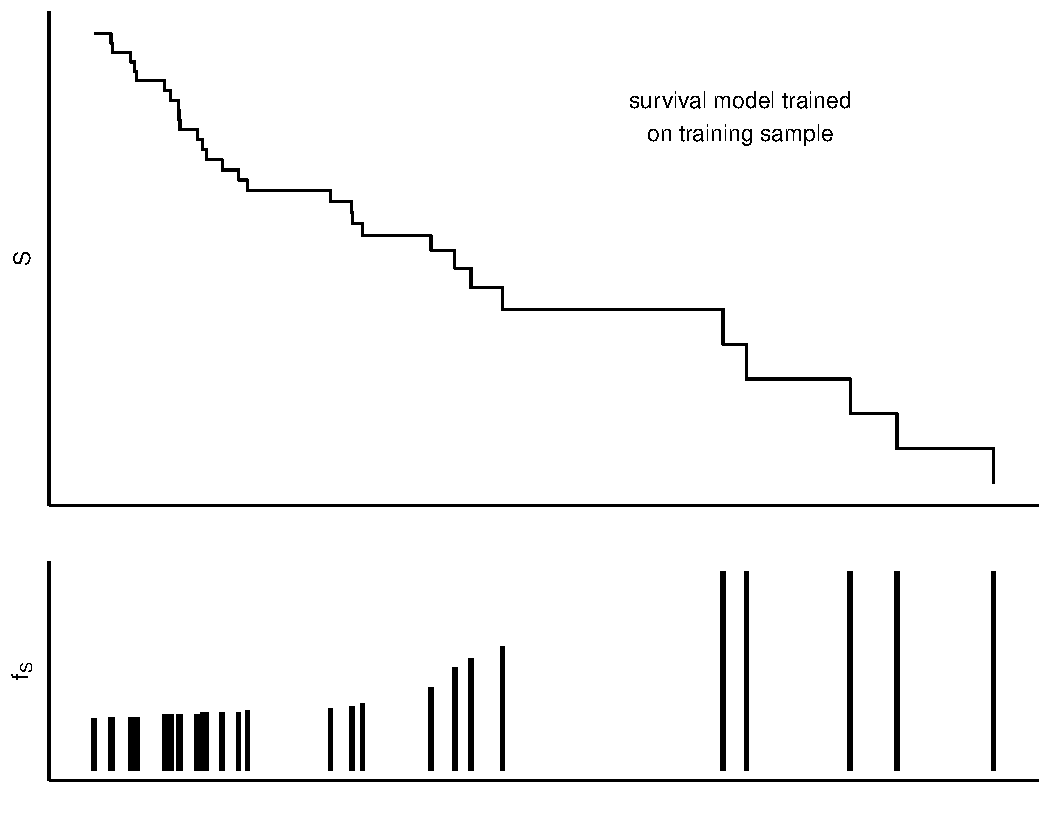
\includegraphics[width=.9\linewidth]{fig-km-surv.pdf}
\end{center}
\end{onlyenv}

\begin{onlyenv}<2>
\begin{center}
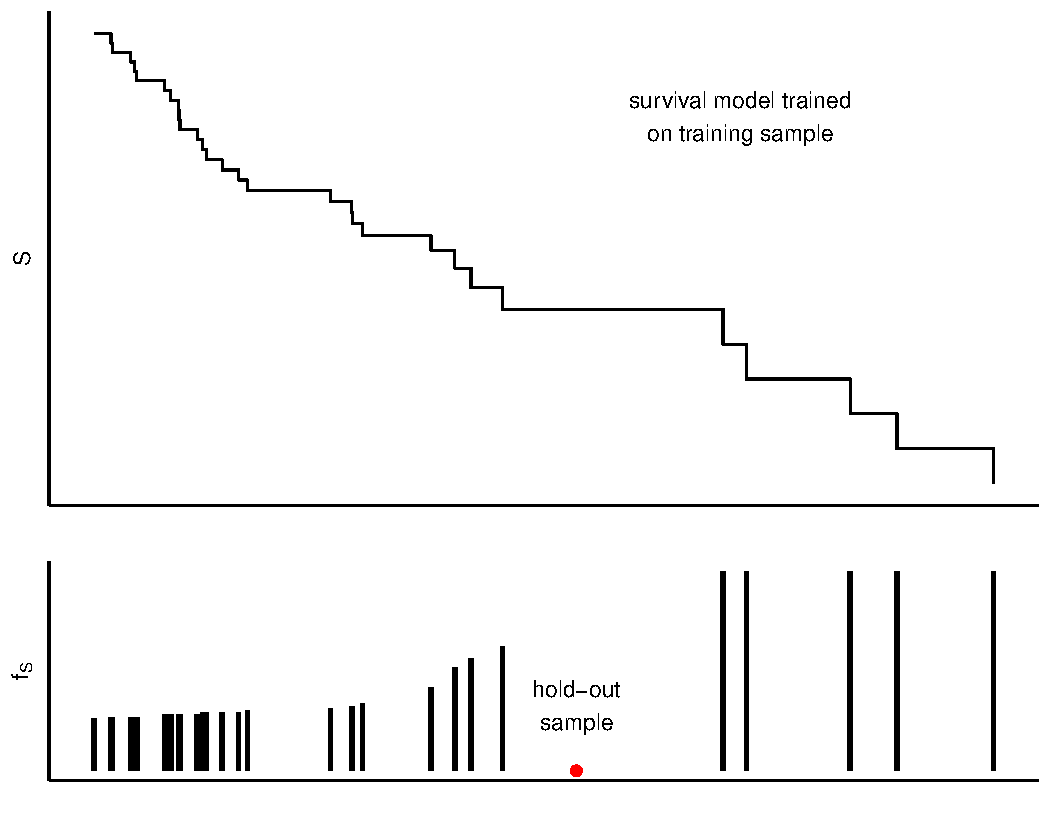
\includegraphics[width=.9\linewidth]{fig-km-surv2.pdf}
\end{center}
\end{onlyenv}
\end{frame}

\begin{frame}[label={sec:orgc4c5bf5}]{Kullback-Leibler divergence and partial likelihoods}
\small Maximum likelihood estimation is connected to minimizing the Kullback-Leibler
divergence and gives an interpretation of the MLE under misspecified models.
\begin{equation*}
  \KL(P_0 \, || \, P) := P_0
  {\left[
      % p_1/p_2
    \log \frac{p_0}{p}
  \right]},
  \quad \text{where} \quad
  P_0 = p_0 \cdot \mu,   P = p \cdot \mu.
\end{equation*}

\begin{onlyenv}<1>
\phantom{With partial likelihood we are minimizing}
\begin{equation*}
 \phantom{  Q \longmapsto \KL(P_{Q_0,G} \, || \, P_{Q,G}), \quad \text{with} \quad Q \in \mathcal{Q}_*.}
\end{equation*}

\vfill

\begin{tikzpicture}
  \draw[line width = .2mm] plot [smooth, tension=.8] coordinates { (0,0) (3,2) (6, 1.2) (9,1)};
  \fill (3,2) circle (0.05);
  \fill (2.6,4) circle (0.05);
  \node[above] (P) at (2.6,4) {\makebox[0pt][l]{$P_0$}\phantom{$P_{Q_0, G}$}};
  \node[] (PP) at (4,.5) {$\mathcal{P}_*$};
  \node[below] (G) at (3,2) {$P_*$};
  \draw[dashed] (3,2) -- (2.6,4);
\end{tikzpicture}
\end{onlyenv}

\begin{onlyenv}<2>
With partial likelihood we are minimizing
\begin{equation*}
  Q \longmapsto \KL(P_{Q_0,G} \, || \, P_{Q,G}),
  \quad \text{with} \quad Q \in \mathcal{Q}_*.
\end{equation*}

\vfill

\begin{tikzpicture}
  \draw[line width = .2mm] plot [smooth, tension=.8] coordinates { (0,0) (3,2) (6, 1.2) (9,1)};
  \fill (3,2) circle (0.05);
  \fill (2.6,4) circle (0.05);
  \node[] (PP) at (4,.5) {$\mathcal{Q}_*$};
  \node[above] (P) at (2.6,4) {$P_{Q_0, G}$};
  \node[below] (G) at (3,2) {$Q_*$};
  \draw[dashed] (2.6,4) -- (3,2);
\end{tikzpicture}
\end{onlyenv}

\begin{onlyenv}<3>
With partial likelihood we are minimizing
\begin{equation*}
  Q \longmapsto \KL(P_{Q_0,G} \, || \, P_{Q,G}),
  \quad \text{with} \quad Q \in \mathcal{Q}_*.
\end{equation*}

\vfill

\begin{tikzpicture}
  \draw[line width = .2mm] plot [smooth, tension=.8] coordinates { (0,0) (3,2) (6, 1.2) (9,1)};
  \node[] (PP) at (4,.5) {$\mathcal{Q}_*$};
  \node[above] (P) at (2.6,4) {$P_{Q_0, G}$};
  \node[above] (P2) at (6.2,3.5) {$P_{Q_0, \tilde{G}}$};
  \node[below] (G) at (3,2) {$Q_*$};
  \node[below] (D) at (6, 1.2) {$\tilde{Q}_*$};
  \draw[dashed] (P2) -- (D);
  \draw[dashed] (2.6,4) -- (3,2);
  \fill (3,2) circle (0.05);
  \fill (2.6,4) circle (0.05);
  \fill (6, 1.2) circle (0.05);
  \fill (6.2,3.5) circle (0.05);
\end{tikzpicture}
\end{onlyenv}
\end{frame}


\begin{frame}[label={sec:org4402c76}]{Inverse probability of censoring weighted loss functions}
\small A conceptually more attractive strategy is to use loss functions that are
\begin{enumerate}[{(i)}]
\item suited for evaluating the performance of estimating the \emph{survival function}
\item defined in terms of the \emph{distribution \(Q\) of interest}
\end{enumerate}

\vfill

We can do this using inverse probability of censoring weighted (IPCW) loss functions. For instance,
with the Brier score
\begin{equation*}
  L_{\mathrm{Brier}}(S, Z) = 
  \left(
    S(t \mid X) - \1
    {\left\{
        T > t
      \right\}}
  \right)^2,
  \quad Z = (T, X) \sim Q,
\end{equation*}
the expected loss is identifiable through
\begin{equation*}
  \E_Q\left[ L_{\mathrm{Brier}}(S, Z) \right]
  = \E_P\left[W_G \cdot L_{\mathrm{Brier}}(S, Z) \right],
\end{equation*}
with
\begin{equation*}
  W_G = \frac{\1{\{\tilde T > t\}} + \1{\{\tilde T \leq t\}}\Delta}{G(\tilde T \wedge t \mid X)},
\end{equation*}
where \(G\) is the conditional ``survivor'' function for the censoring distribution
\citep{graf1999assessment,gerds2006consistent,van2003unicv}.
\end{frame}


\begin{frame}[label={sec:org1c1f34f}]{Estimation of the IPC weights}
\small

To use IPCW loss functions in practice we need to estimate \(G\). This is the same estimation
problem as estimation of \(S\), just with the meaning of \(\Delta\) reversed. 

\vfill

\(\implies\) The exact same challenges face us when attacking this problem.

\vfill

\def\shift{2.3}
\def\ls{}
\def\lw{.5mm}
\begin{center}
\begin{tikzpicture}
  \node[] (S) at (0,\shift) {$\hat S$};
  \node[] (WG) at (\shift,\shift) {$W_{\hat G}$};
  \node[] (G) at (\shift,0) {$\hat G$};
  \node[] (WS) at (0,0) {$W_{\hat S}$};
  \draw[<-, \ls, line width=\lw, cyan] (S) to[out=30,in=150] (WG);
  \draw[<-, \ls, line width=\lw, cyan] (WG) to[out=30-90,in=150-90] (G);
  \draw[<-, \ls, line width=\lw, cyan] (G) to[out=30-180,in=150-180] (WS);
  \draw[<-, \ls, line width=\lw, cyan] (WS) to[out=30-270,in=150-270] (S);
\end{tikzpicture}
\end{center}

\vfill

Recently, \cite{han2021inverse} and \cite{westling2021inference} have suggested to iterate between
estimation of \(\hat S\) and \(\hat G\) until convergence.
\end{frame}


\section{Double robustness and fluctuation risk}
\label{sec:org85dfb91}
\begin{frame}[label={sec:org52e2c82}]{}
\begin{block}{\centering Not obvious how to select our survival model}
\pause
\end{block}
\begin{block}{}
\end{block}
\begin{beamercolorbox}[rounded=true]{gray}
\centering When \(S\) is a nuisance parameter we could aim at selecting the model based on a
criteria designed for the parameter of interest. \pause
\end{beamercolorbox}

\begin{block}{}
\end{block}

\begin{block}{Exploiting double robustness}
\cite{tchetgenYifanTagetDML}, building on ideas from \cite{robins2007comment}, proposed to exploit
double robustness as a model selection criteria.
\end{block}
\end{frame}


\begin{frame}[label={sec:org79ef8c7}]{Fluctuation risk}
Let \(\psi\) be the efficient influence for the parameter \(\Psi\), and assume we can write \(\psi(O, P)
= \phi(O, S_P, G_P) - \Psi(P)\) such that
\begin{equation*}
  \E_P{\left[ \phi(O, S_P, G_*) \right]}
  = \E_P{\left[ \phi(O, S_*, G_P) \right]}
  = \Psi(P),
\end{equation*}
for any \(S_*\) and \(G_*\), where \(S_P\) and \(G_P\) are the conditional survivor functions
corresponding to the data generating distribution.

\vfill \pause

\small Let \(\mathcal{G}\) be a (finite) collection of models for \(G\). The double robustness
property implies that 
\(\E_P{\left[ \phi(O, S_P, G) \right]} = \E_P{\left[ \phi(O, S_P, G') \right]}\) for any
\(G, G' \in \mathcal{G}\). In particular,
\begin{equation*}
  \max_{G, G' \in \mathcal{G}}\big\vert
  \E_P{\left[ \phi(O, S_P, G) \right]}
  - \E_P{\left[ \phi(O, S_P, G') \right]}     
  \big\vert
  = 0.
\end{equation*}
\pause This motivates the ``fluctuation risk'',\footnote<3>{or pseudo-risk because it depends \(\mathcal{G}\) which is suppressed in the notation.}
\begin{equation*}
  % \label{eq:dr}
  R(S)
  =
  \max_{G, G' \in \mathcal{G}}\big\vert
  \E_P{\left[ \phi(O, S, G) \right]}
  - \E_P{\left[ \phi(O, S, G') \right]}     
  \big\vert.
\end{equation*}
\end{frame}

\begin{frame}[label={sec:org50ab19a}]{Estimating the fluctuation risk}
Let $\mathcal{A}_c$ be a collection of algorithms for estimating \(G\). For any $\nu \in \mathcal{A}$,
$\gamma \in \mathcal{A}_c$, and \(k = 1, \dots, K\) define
\begin{equation*}
  \hat{\Psi}_{\nu, \gamma}^k =
  \frac{1}{|D_k|} \sum_{O \in D_k}
  \phi(O, \nu(D_{-k}), \gamma(D_{-k})).
\end{equation*}
For any $\nu \in \mathcal{A}$ we approximate the fluctuation risk with
\begin{equation*}
  \hat R(\nu) =
  \frac{1}{K}
  \sum_{k=1}^{K}
  \max_{\gamma, \gamma' \in \mathcal{A}_c}
  \big|\hat{\Psi}_{\nu, \gamma}^k -
  \hat{\Psi}_{\nu, \gamma'}^k\big|.  
\end{equation*}
% and select our final nuisance estimator as
% \begin{equation*}
%   \argmin_{\nu \in \mathcal{A}} R(\nu).
% \end{equation*}
% (We use a similar strategy to pick $\gamma \in \mathcal{A}_c$.)

\vfill

Recall
\begin{description}
\item[{\(\mathcal{A}\)}] collection of algorithms for estimating \(S \in \mathcal{S}\)
\item[{\(D_1, \dots, D_K\)}] partition of the data set \(D\)
\item[{\(D_{-k}\)}] the \(k\)'th training sample, \(D_{-k} = D \setminus D_{k}\), \(k=1, \dots, K\)
\end{description}
\end{frame}

\begin{frame}[label={sec:orgf0d774f},fragile]{Illustration of the method}
 \begin{onlyenv}<1>
\small Consider the following simple setting where \(X=(A_1, A_2, A_3)^T\) with \(A_j \in \{0,1\}\)
for all \(j\) and our parameter of interest is the marginal survival probability \(Q(T > t)\) at
some fixed time \(t>0\). We consider using Kaplan-Meier estimators stratified on each of
\(A_j\).\footnote{In this simulation, only \(A_1\) influences survival and censoring.}

\vspace{.4cm}

\begin{block}{\centering outcome algorithms}
\lstset{language=r,label= ,caption= ,captionpos=b,numbers=none}
\begin{lstlisting}
S1 <- function(d) prodlim(Surv(time,event) ~ A1, data = d)
S2 <- function(d) prodlim(Surv(time,event) ~ A2, data = d)
S3 <- function(d) prodlim(Surv(time,event) ~ A3, data = d)
\end{lstlisting}
\end{block}

\begin{block}{\centering censoring algorithms}
\lstset{language=r,label= ,caption= ,captionpos=b,numbers=none}
\begin{lstlisting}
G1 <- function(d) prodlim(Surv(time,event) ~ A1, rev = T, data = d)
G2 <- function(d) prodlim(Surv(time,event) ~ A2, rev = T, data = d)
G3 <- function(d) prodlim(Surv(time,event) ~ A3, rev = T, data = d)
\end{lstlisting}
\end{block}
\end{onlyenv}

\begin{onlyenv}<2->
\begin{onlyenv}<2>
\begin{center}
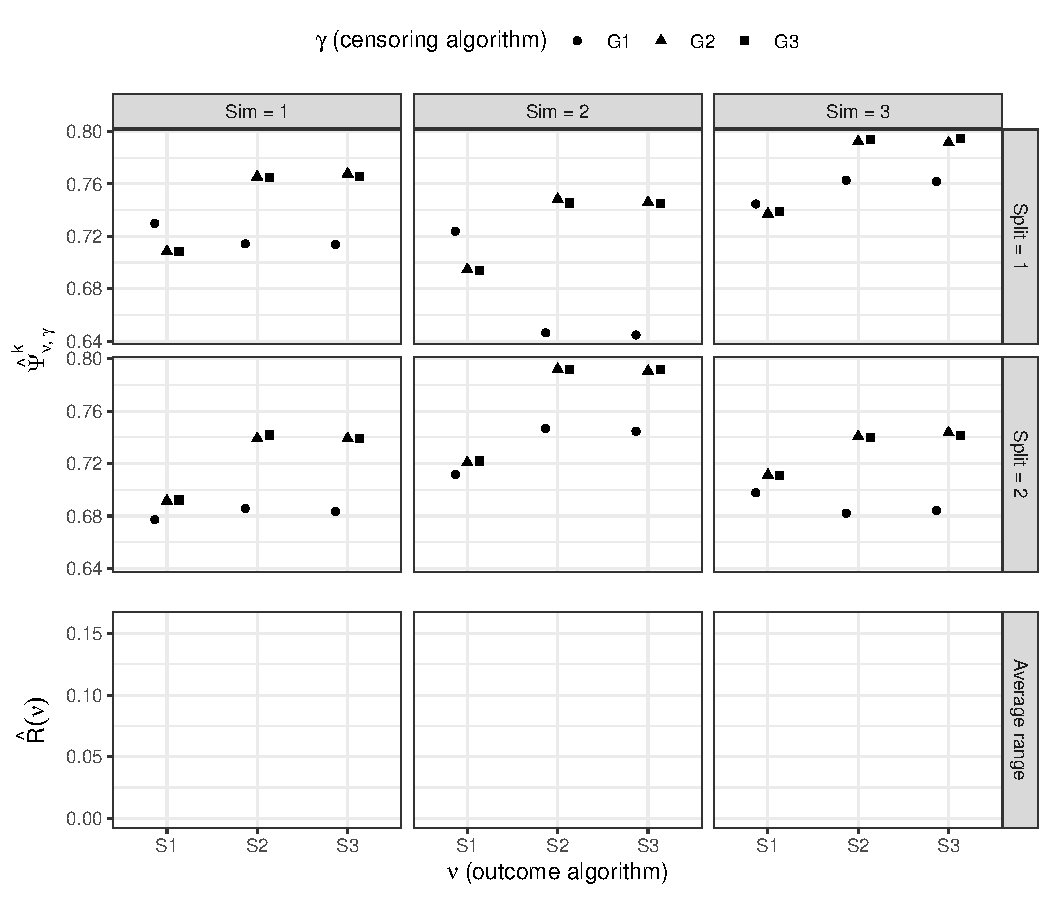
\includegraphics[width=.9\linewidth]{fig-illustrate-fluct-risk.pdf}
\end{center}
\end{onlyenv}

\begin{onlyenv}<3>
\begin{center}
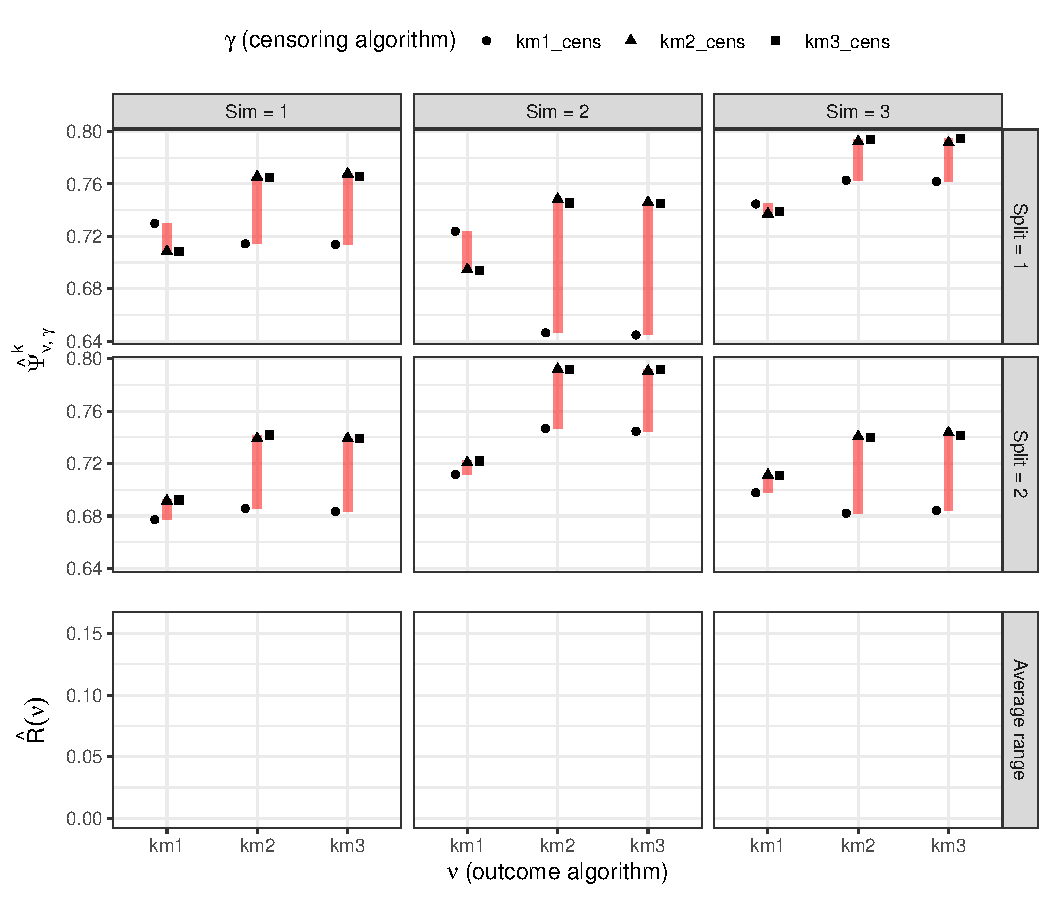
\includegraphics[width=.9\linewidth]{fig-illustrate-fluct-risk2.pdf}
\end{center}
\end{onlyenv}

\begin{onlyenv}<4>
\begin{center}
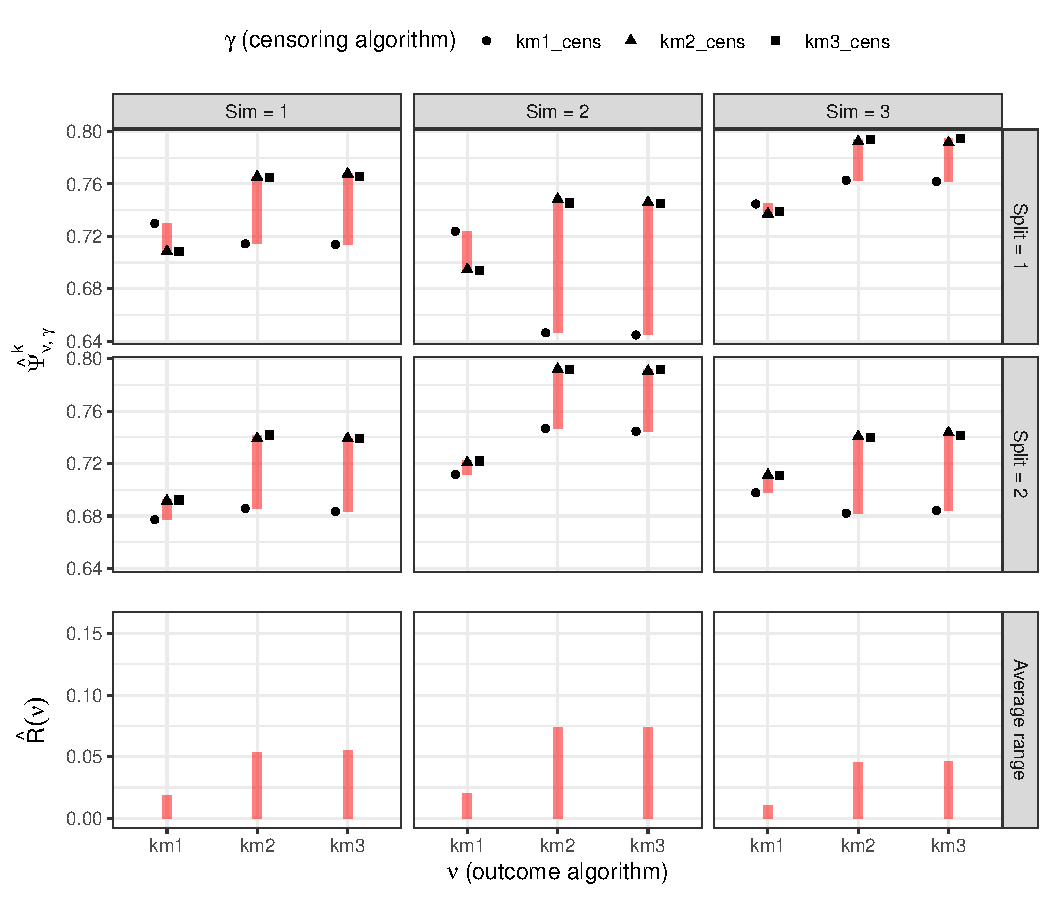
\includegraphics[width=.9\linewidth]{fig-illustrate-fluct-risk3.pdf}
\end{center}
\end{onlyenv}
\end{onlyenv}
\end{frame}

\begin{frame}[label={sec:org0a15466}]{Some simulation results}
\begin{onlyenv}<1>
\begin{center}
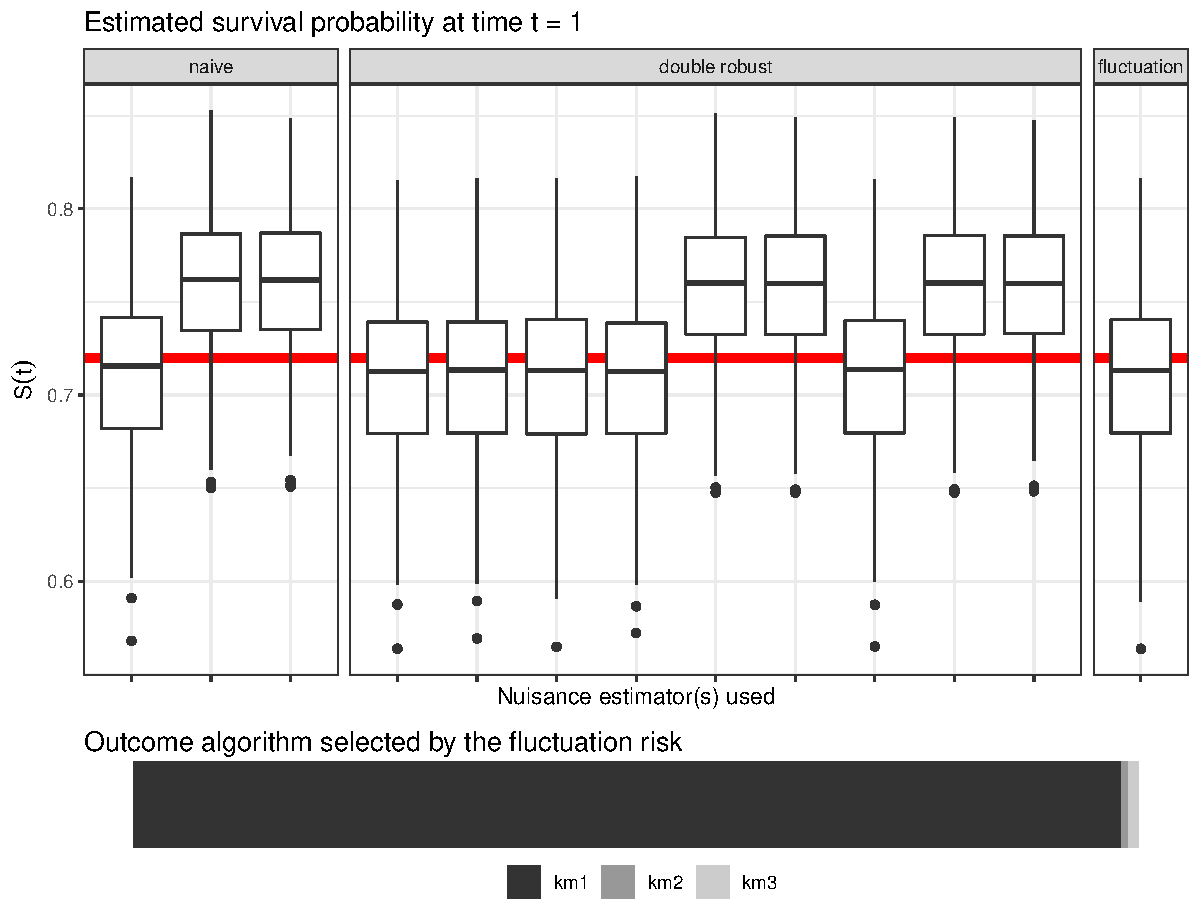
\includegraphics[width=.9\linewidth]{sim-results1.pdf}
\end{center}
\end{onlyenv}


\begin{onlyenv}<2>
\begin{center}
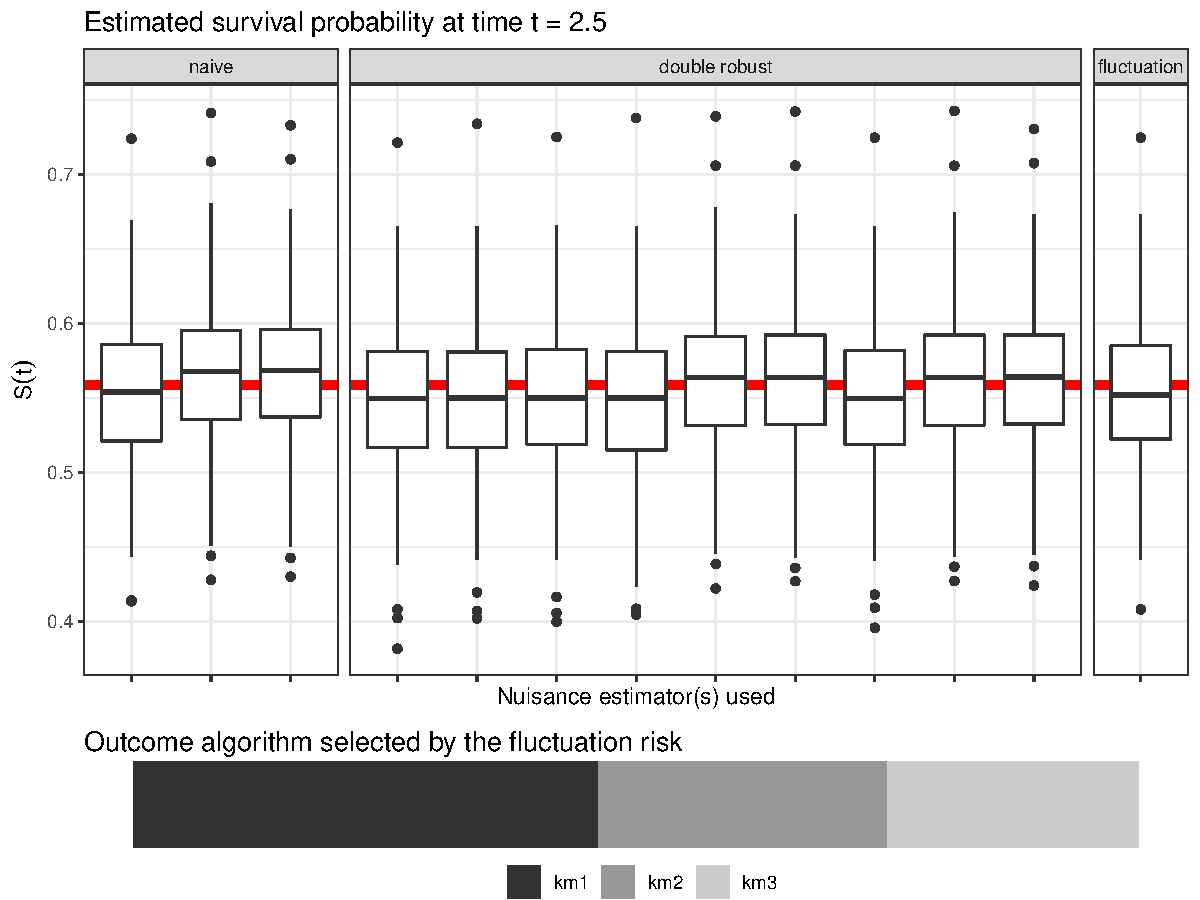
\includegraphics[width=.9\linewidth]{sim-results2.pdf}
\end{center}
\end{onlyenv}
\end{frame}

\begin{frame}[label={sec:orgb96db80}]{Conclusion}
\begin{itemize}
\item It is not obvious what loss function to use for estimating the conditional survivor function with
censored data observed in continuous time.
\item If the parameter of interest is a low-dimension feature of the full data distribution we could
exploit this and evaluate the performance of the nuisance parameter estimators in terms of their
effect on the estimator of the target parameter.
\end{itemize}
\end{frame}

\section*{References}
\label{sec:orgcb1724d}
\begin{frame}[label={sec:org9311b7f}]{References}
\footnotesize \bibliography{./latex-settings/default-bib.bib}
\end{frame}
\section*{Appendix}
\label{sec:org4aa5a41}
\appendix
\begin{frame}[label={sec:orgd27c608}]{If the conditional survivor function was the target parameter}
\small Consider now the situation where the conditional survival function \(S(t \mid x)\) is the
actual parameter of interest for fixed \(t\). Assume that our goal is to build a prediction model
minimizing the average Brier score. Given a model \(S\) we can consider the average
Brier score of \(S\) as a low dimensional target parameter
\begin{equation*}
  \Psi_S(P) = \E_P{\left[ W_G \cdot L_{Brier}(S, Z) \right]}
  \quad \text{with} \quad G = G_P,
\end{equation*}
and proceed as above.

\begin{itemize}
\item With a finite \emph{collection} of models \(\mathcal{S}^*\subset\mathcal{S}\) we get a different target parameter \(\Psi_S\)
for each \(S \in\mathcal{S}^*\).
\item With an infinite collection of models \(\mathcal{S}^*\) (e.g., indexed by \(\beta \in \R^p\)) the
previous approach is problematic.
\end{itemize}

\(\implies\) It is desirable to fit the weights \emph{once} so that they are ``universally''
applicable for estimating the performance of all \(S \in \mathcal{S}\).

\vfill

One idea is to use undersmoothed HAL to do this.
\end{frame}
\end{document}